\documentclass[]{AO4ELT}  %>>> use for US letter paper
%\documentclass[a4paper]{AO4ELT}  %>>> use this instead for A4 paper
%\documentclass[nocompress]{AO4ELT}  %>>> to avoid compression of citations

\renewcommand{\baselinestretch}{1.0} % Change to 1.65 for double spacing
\usepackage{microtype}
\usepackage{biblatex}
\usepackage{amsmath,amsfonts,amssymb}
\usepackage{graphicx}
%\usepackage{pst-all} % Pour pstricks
\usepackage[colorlinks=true, allcolors=blue]{hyperref}
% \addbibresource{report.bib}

% Definition of \maketitle
\makeatletter         
\def\@maketitle{
%\raggedleft

\includegraphics[width = 170mm]{ao4elt_logo_vf.png}\\[8ex]
\begin{center}
{\Huge \bfseries \sffamily \@title }\\[4ex] 
{\Large  \@author}\\[4ex] 
\@date%\\[8ex]
\end{center}}
%\makeatother





\title{GMT Natural Guide Star Adaptive Optics Integrated Modeling}

\author[a]{R.~Conan, R.~Romano, C.~Dribusch, K.~Vogiatzis, H.~Fitzpatrick, M.~Shabram, B.~Walls, B.~Sitarski, A.~Bouchez, F.~Quiros-Pacheco, P.~Thompson, H.~Chiquito, K.-M.~Lam, D.~Ashby, T.~Ranka}
%\author[b]{Léon Foucault}
\affil[a]{GMTO}
%\affil[b]{Affiliation2, Address, City, Country}

\authorinfo{Further author information: (Send correspondence to J.M.O.)\\J.F.G.: E-mail: jfg@adaptiveoptics.edu, Telephone: 1 505 123 1234\\  L.F.: E-mail: fourier@transform.com, Telephone: +33 (0)1 05 49 25 32}





% Option to view page numbers
\pagestyle{empty} % change to \pagestyle{plain} for page numbers   
\setcounter{page}{301} % Set start page numbering at e.g. 301

\graphicspath{{figures}}

\begin{document}
\maketitle
\begin{abstract}
   The Giant Magellan Telescope Project relies on a comprehensive integrated modeling tool to evaluate Observatory Performance Modes, ranging from Seeing Limited to Adaptive Optics. This STOP (Structural-Thermal-Optical Performance) model includes the dynamics of each domain-specific model, accounting for time-varying disturbances such as wind jitter, vibrations, and temperature fluctuations. However, creating such a model presents challenges due to the wide range of scientific and engineering expertise required, as well as the large number of degrees of freedom to handle. Adaptive Optics presents additional challenges due to its high sampling rate of 1kHz or more, exacerbated by the need to simulate long science exposures under various operating conditions.
   This paper will introduce the main components of the integrated model, including finite element, optical, control, and computational fluid dynamics, as well as the stringent verification and experimental validation processes that the model undergoes. The choice of computing framework that integrates domain-specific models into a unified model is critical and will be described in detail. The development of the integrated model is driven by the need to accurately estimate errors that affect the science instrument data products and mitigate technological risks associated with the telescope. Examples will be given on how the error budgets and risk register are used to set priorities for the integrated modeling simulations queue.
   The GMTO project has identified a set of Key Performance Parameters (KPP) that summarize the expected performance for each Observatory Performance Mode. These KPPs are statistical quantities derived from Monte-Carlo simulations of the Observatory under various operating and environmental conditions. This paper will show how Monte-Carlo simulations have been performed at the Observatory level for the Natural Guide Star Adaptive Optics OPM.
\end{abstract}

% Include a list of keywords after the abstract 
\keywords{Extremely Large Telescope, Adaptive Optics, Integrated Model}

\section{INTRODUCTION}
\label{sec:intro}


The Giant Magellan Telescope (Fig.~\ref{fig:1}) is a 25.5 diameter Gregorian aplanatic optical segmented telescope.
Both the primary and the secondary mirrors are made of 7 circular segments collocated on the alt-az telescope mount.
The focal plane is located below the center segment of the primary mirror where a carousel of scientific instruments is implemented.
The secondary mirror can be fitted with 7 adaptive secondary mirrors (ASM), each one 1m in diameter and which shape is controlled with 675 actuators.
The seven ASMs enable the Adaptive Optics (AO) Observing Modes of the telescope i.e. Natural Guide Star (NGAO), Laser Tomography (LTAO) and Ground Layer (GLAO).

The GMT project has defined a set of optical performance requirements for each Observing Modes.
The GMT Integrated Model is used to assess the compliance of the telescope with respect to the performance requirements.
The integrated model (Fig.\ref{fig:2}) is a composition of different models that emulates the Structural-Thermal-Optical dynamics of the telescope.

The NGAO Integrated Model of the GMT (Fig.~\ref{fig:4}) is based on the traditional AO model (Fig.~\ref{fig:3}).
But it includes as well, the telescope structural dynamic model, the details of the control system for the mount, the primary mirror and the secondary mirror,
ray-tracing through the telescope and the dynamics of wind loads and enclosure dome seeing.

%\begin{itemize}
%   \item End-To-End model
%   \item Structural-Thermal-Optical Performance (STOP) model
%   \item Transient STOP (T-STOP) model
%   \item Computer Assisted Assembly Integration \& Verification
%\end{itemize}

\begin{figure}
   \centering
   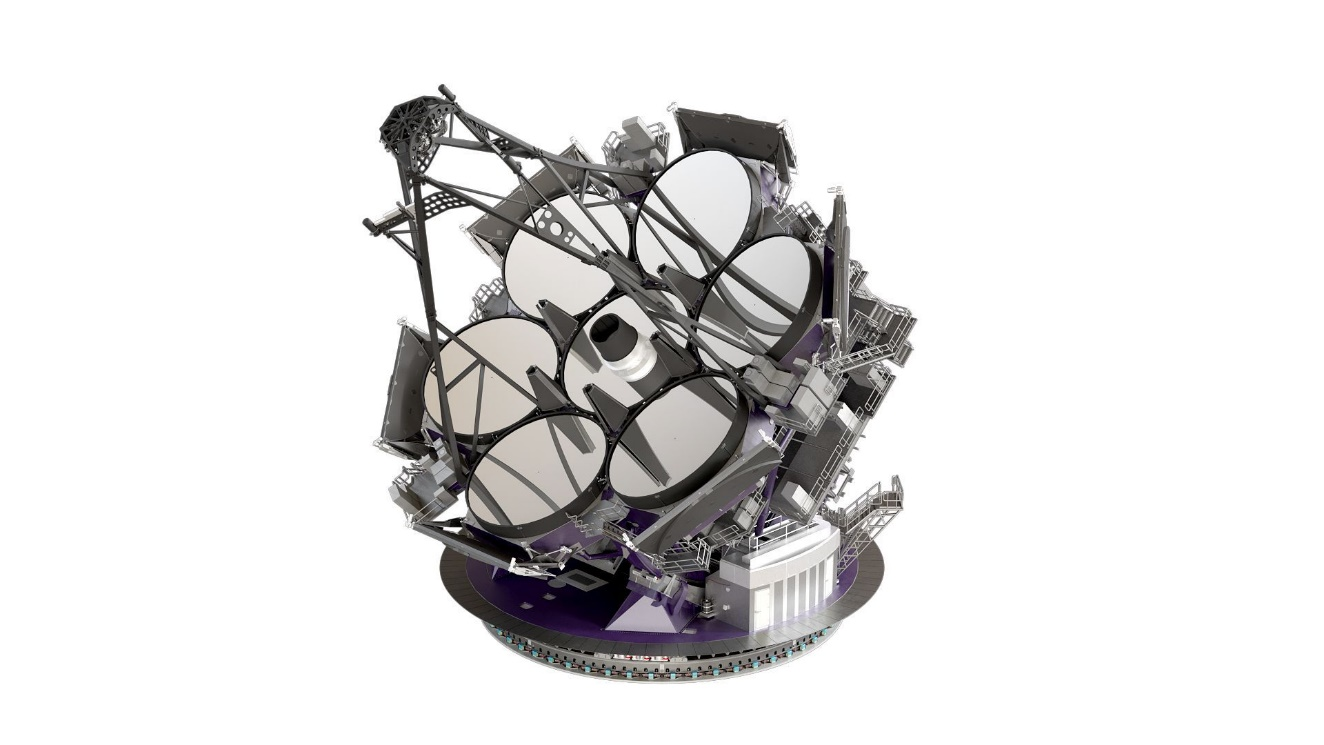
\includegraphics[trim=8cm 1cm 9cm 2cm,clip,scale=0.6]{./figures/gmt-pretty.png}
   \caption{GMT 3D rendering.}
   \label{fig:1}
\end{figure}

\begin{figure}
   \centering
   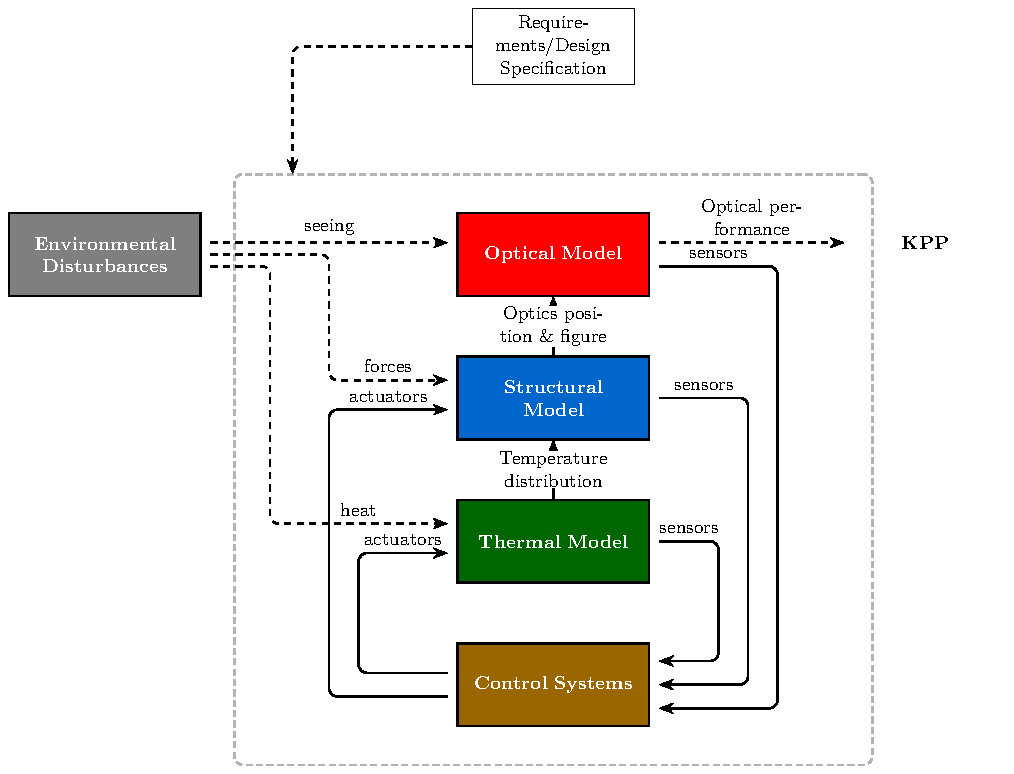
\includegraphics[width=0.9\linewidth]{./figures/integrated_modeling-bare.pdf}
   \caption{GMT Integrated Model.}
   \label{fig:2}
\end{figure}

\begin{figure}
   \centering
   \includegraphics[width=0.7\linewidth]{./figures/{end2end_ngao-only.drawio}.png}
   \caption{Adaptive Optics Block Diagram.}
   \label{fig:3}
\end{figure}

\begin{figure}
   \centering
   \includegraphics[width=\linewidth]{./figures/{end2end_ngao-ngao-im-e2e.drawio}.png}
   \caption{Adaptive Optics Integrated Model Block Diagram.}
   \label{fig:4}
\end{figure}

\clearpage

\section{GMT INTEGRATED MODEL}
\label{seg:gmt-im}

\subsection{Computational Fluid Dynamics \& Thermal Models}
\label{sec:cfd}

A comprehensive suite of computational fluid dynamics (CFD) \& thermal models (Fig.~\ref{fig:5}) have been developed for the GMT.
The models are inter--dependent meaning that the outputs of some models serves as thermal boundary conditions for the others.
Thermal phenomenon varies slowly with time compare to the rapid changes in the atmospheric turbulence for example.
So in the context of the GMT NGAO IM, the thermal perturbations are static inputs except for wind loads and dome seeing.

A detailed CFD model of the Observatory has been developed (Fig.~\ref{fig:6}) that includes the mountain summit
with the telescope and the auxiliary support buildings.
The CFD model computes, inside the telescope enclosure, the random fields of temperature and pressure (Fig.~\ref{fig:7}).
From the pressure field, the forces and torques (Fig.~\ref{fig:8a}) applied at several locations on the telescope structure is derived and
from the temperature field, the random field of the air index of refraction is derived.
The integration of the index of refraction along the optical path through the telescope
to the exit pupil leads to the dome seeing wavefront error map (Fig.~\ref{fig:8b}).

\begin{figure}
   \centering
   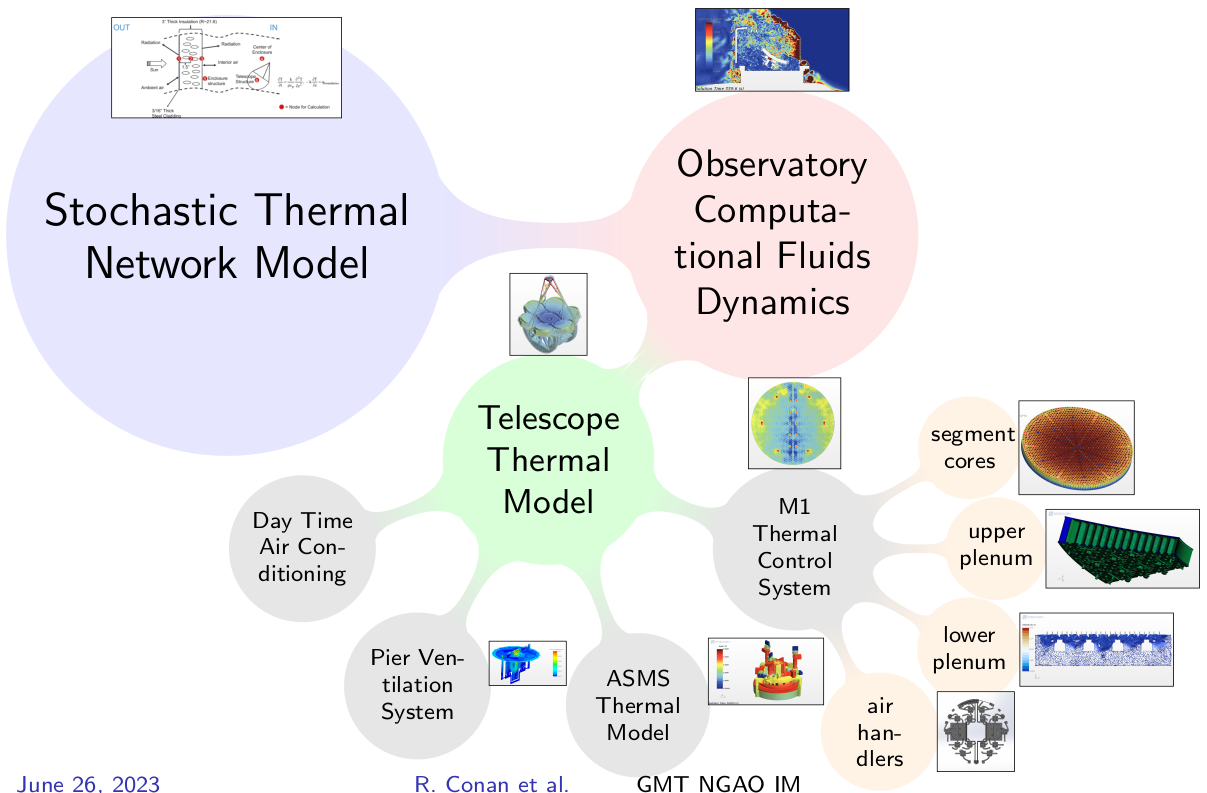
\includegraphics[width=0.7\linewidth]{./figures/cfd-thermal_models.png}
   \caption{GMT CFD \& Thermal models.}
   \label{fig:5}
\end{figure}

\begin{figure}
   \centering
   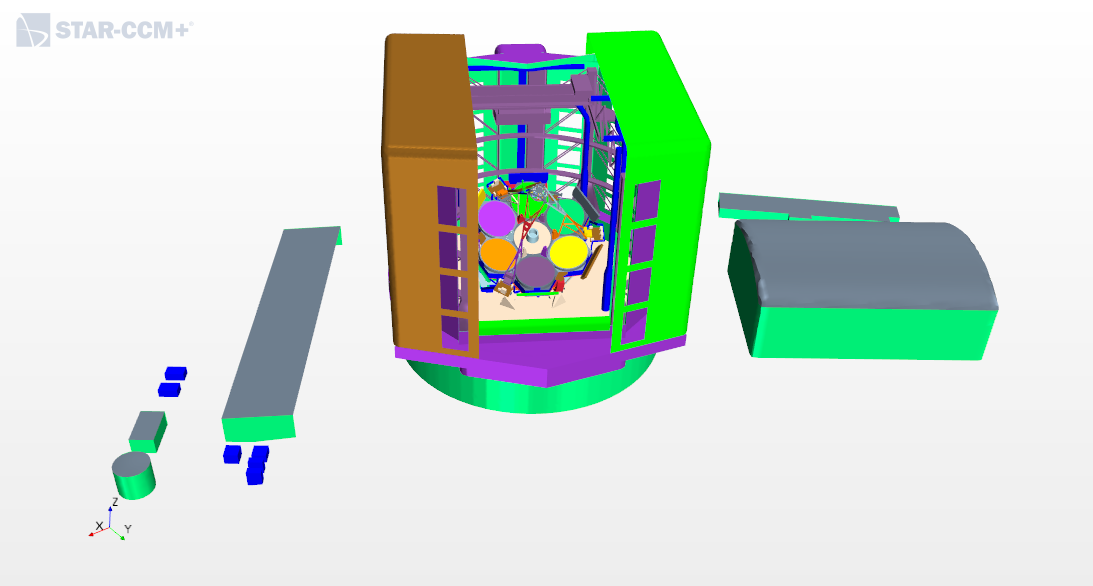
\includegraphics[trim= 0 0 0 2cm,clip,width=0.95\linewidth]{./figures/zen30az000_OS7_Geometry Scene 2.png}
   \caption{GMT Observatory CFD model.}
   \label{fig:6}
\end{figure}

\begin{figure}
   \centering
   \includegraphics[width=0.495\linewidth]{./figures/{vort_tel_vort_tel_3.000000e+02}.png}
   \includegraphics[width=0.495\linewidth]{./figures/{RI_tel_RI_tel_3.000000e+02}.png}
   \caption{Vorticity \& Gradient of index of refraction.}
   \label{fig:7}
\end{figure}

\begin{figure}
   \centering
   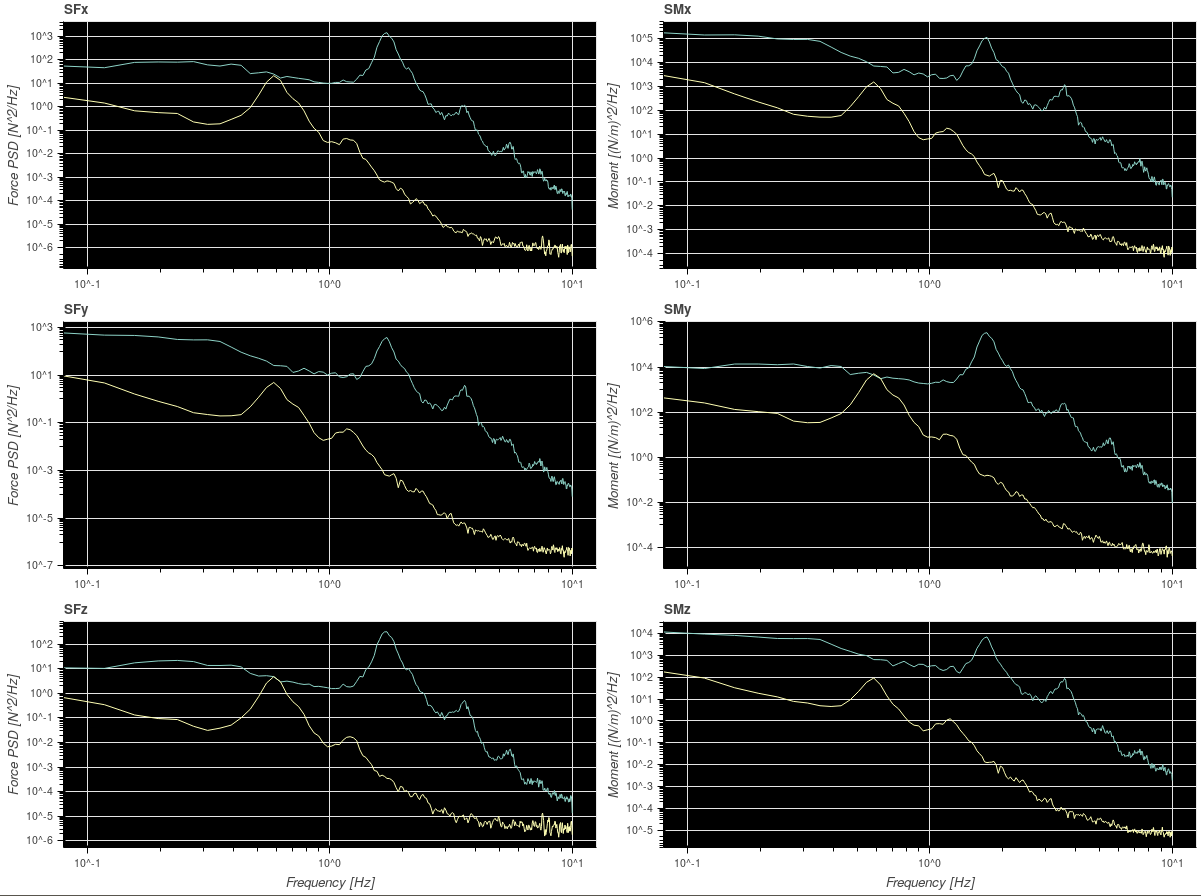
\includegraphics[width=0.7\linewidth,trim=0 21cm 21cm 1cm,clip]{./figures/FM_PSDs.png}
   \caption{Forces PSD w/ evidence of vortex shedding}
   \label{fig:8a}
\end{figure}
\begin{figure}
   \centering
   \includegraphics[width=0.6\linewidth]{./figures/{opd.mp4}.png}
   \caption{Dome Seeing OPD (PTV $\pm 3\mu$m).}
   \label{fig:8b}
\end{figure}

\clearpage

\subsection{Structural Dynamic Model}
\label{sec:fem}

A structural dynamic model is a linear combination of 2nd order differential equations.
\begin{eqnarray*}
   \label{eq:1}
   && \ddot q_i + 2\zeta_i \omega_i \dot q_i + \omega_i^2 q = b_i u \\
   && y = c_i q_i
\end{eqnarray*}
Each equation (Eq.~\ref{eq:1}) represents the dynamic of a mode of the system
where
\begin{itemize}
   \item $u$: force \& torque inputs,
   \item $y$: node position outputs,
   \item eigen mode: $q_i$, eigen frequency $w_i$, damping coefficient: $\zeta_i$,
   \item $b_i$, $c_i$: nodal (zonal) to modal linear transformation.
\end{itemize}

\begin{figure}
   \centering
   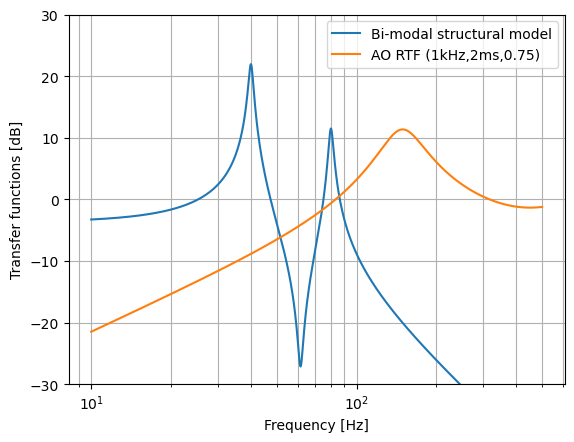
\includegraphics[width=0.5\linewidth]{./figures/bi-modal_sm.png}
   \caption{Bi-modal structural model with the rejection transfer function of a typical Adaptive Optics for comparison.}
   \label{fig:90}
\end{figure}

An example of a bi-modal structural dynamic model is given in Fig.~\ref{fig:90}.
In practice, a structural system is made of thousands of modes as shown in the transfer function of the mount (Fig.~\ref{fig:9}).
This leads to the presence a multiple resonance frequencies in the system.
The mechanical structure then acts like a resonator where vibration sources may couple to some resonant eigen modes.

\subsubsection{Structural Model Frequency Responses}
\label{sec:fem-frequency}

\begin{figure}
   \centering
   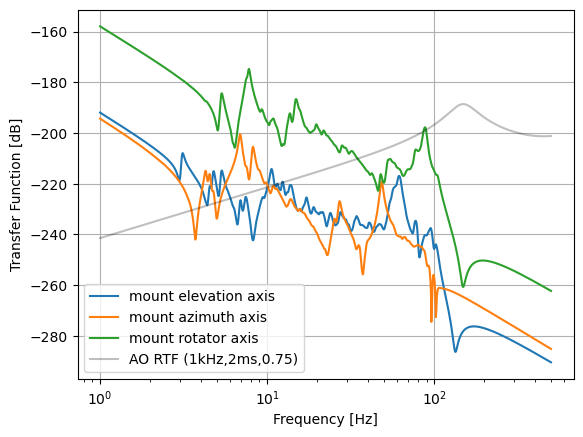
\includegraphics[width=0.495\linewidth]{./figures/mount-axis-tfs.png}
   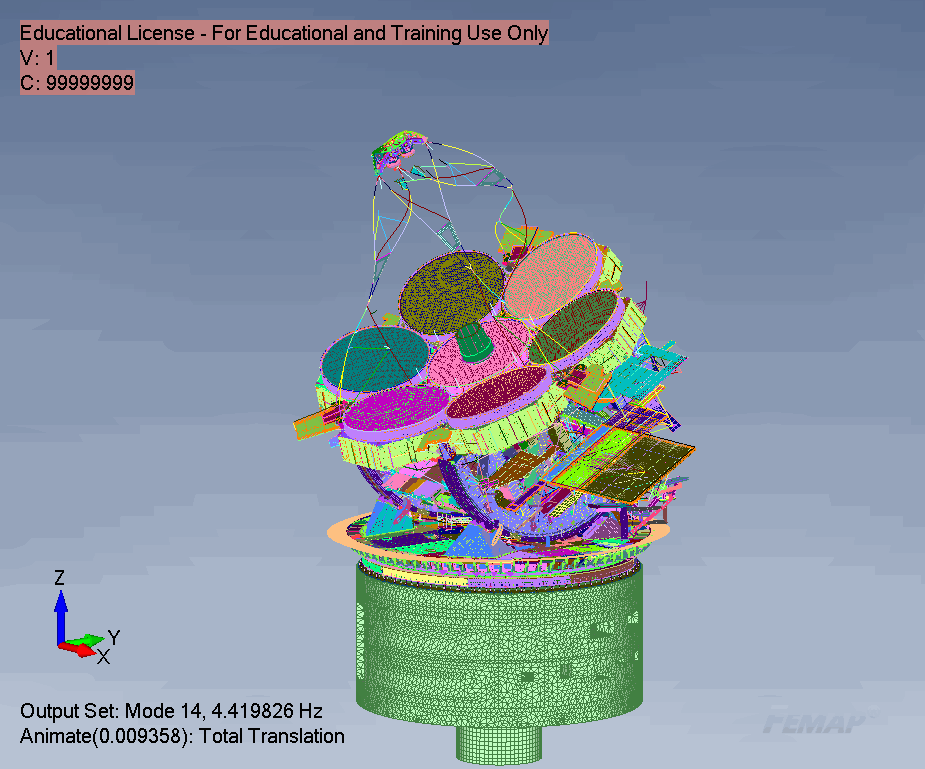
\includegraphics[width=0.4\linewidth]{./figures/fem-mode-9.png}
   \caption{GMT Mount Drives to Encoders SISO (Single Input Single Ouput) Transfer Functions.}
   \label{fig:9}
\end{figure}

\subsubsection{Control Structure Interactions}
\label{sec:fem-csi}

\begin{itemize}
   \item \emph{ASM dynamics model} (P. Thompson (GMT) \& M. Manetti (Adoptica)) including \emph{fluid damping}
   \item \emph{voice coils position} to \emph{thin shell figure} MIMO ($675\times 675$) transfer function
\end{itemize}
\begin{itemize}
   \item projection of symptomatic eigen mode onto Karhunen-Loeve (KL) basis
   \item KL to KL SISO transfer function
\end{itemize}

\begin{itemize}
   \item \emph{ASM dynamics model} (P. Thompson (GMT) \& M. Manetti (Adoptica)) including \emph{fluid damping}
   \item \emph{voice coils position} to \emph{thin shell figure} MIMO ($675\times 675$) transfer function
\end{itemize}

\begin{figure}
   \centering
   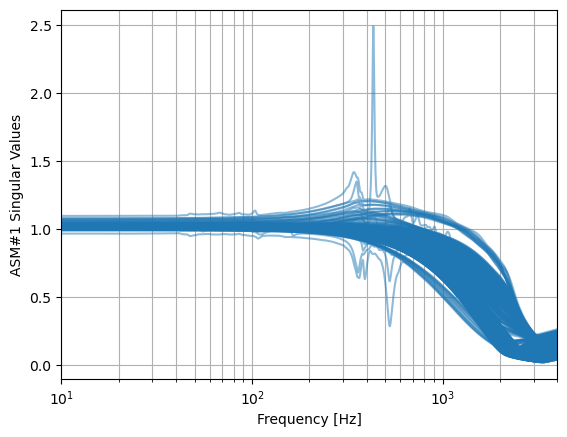
\includegraphics[width=0.6\linewidth]{./figures/asm-mimo-svd.png}
   \caption{GMT ASM Zonal MIMO (Multi-Input Multi-Ouput) Transfer Function singular values as a function of frequencies.}
   \label{fig:10}
\end{figure}

\begin{figure}
   \centering
   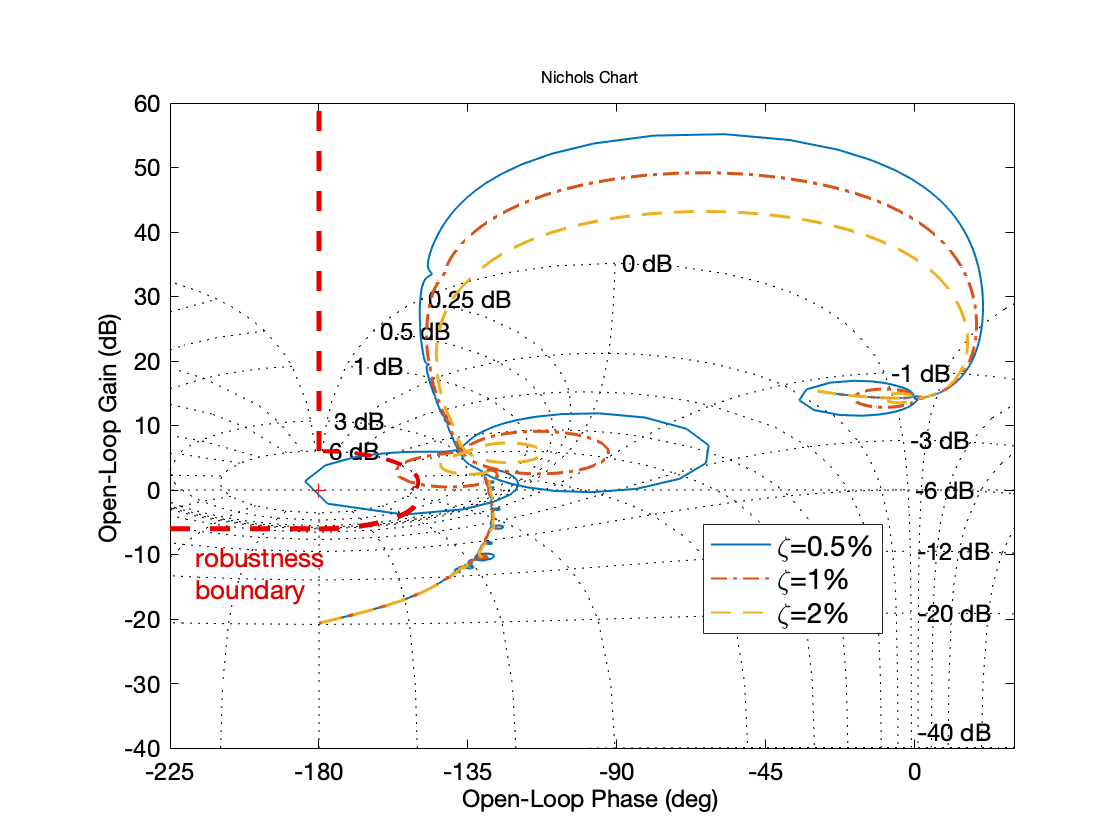
\includegraphics[trim=3cm 0 0 3cm,clip,width=0.6\linewidth]{./figures/defocusNicholsLTF.png}
   \caption{Nichols plot of focus mode versus damping $\zeta$.}
   \label{fig:11}
\end{figure}

\clearpage

\subsection{Optical Model}
\label{sec:optics}

The optical model, CEO (Cuda-Engined-Optics), is a GPU-based ray tracing and Fourier propagation model that propagates a collimated light beam to the telescope focal plane (Fig.~\ref{fig:12}),
first by ray tracing to the telescope exit pupil and then Fourier propagating the light to a detector image plane.

CEO also have models for all the wavefront sensors that are used on the GMT like the pyramid wavefront sensor (Fig.~\ref{fig:13}) and the holographic dispersed fringe sensor (HDFS) (Fig.~\ref{fig:14}).

%\begin{itemize}
%   \item ray tracing to the exit pupil
%   \item Fourier propagation to detector image plane
%   \item NGAO wavefront sensors \cite{F. Quiros, "NGAO \& GMT Phasing"}\cite{B. Sitarski, "GMT HDFS"}\cite{C. Plantet, "GMT NGWFS Prototype"}:
%         \begin{itemize}
%            \item $96\times 96$ pyramid wavefront sensor
%            \item holographic dispersed fringe sensor (HDFS)
%         \end{itemize}
%\end{itemize}

\begin{figure}
   \centering
   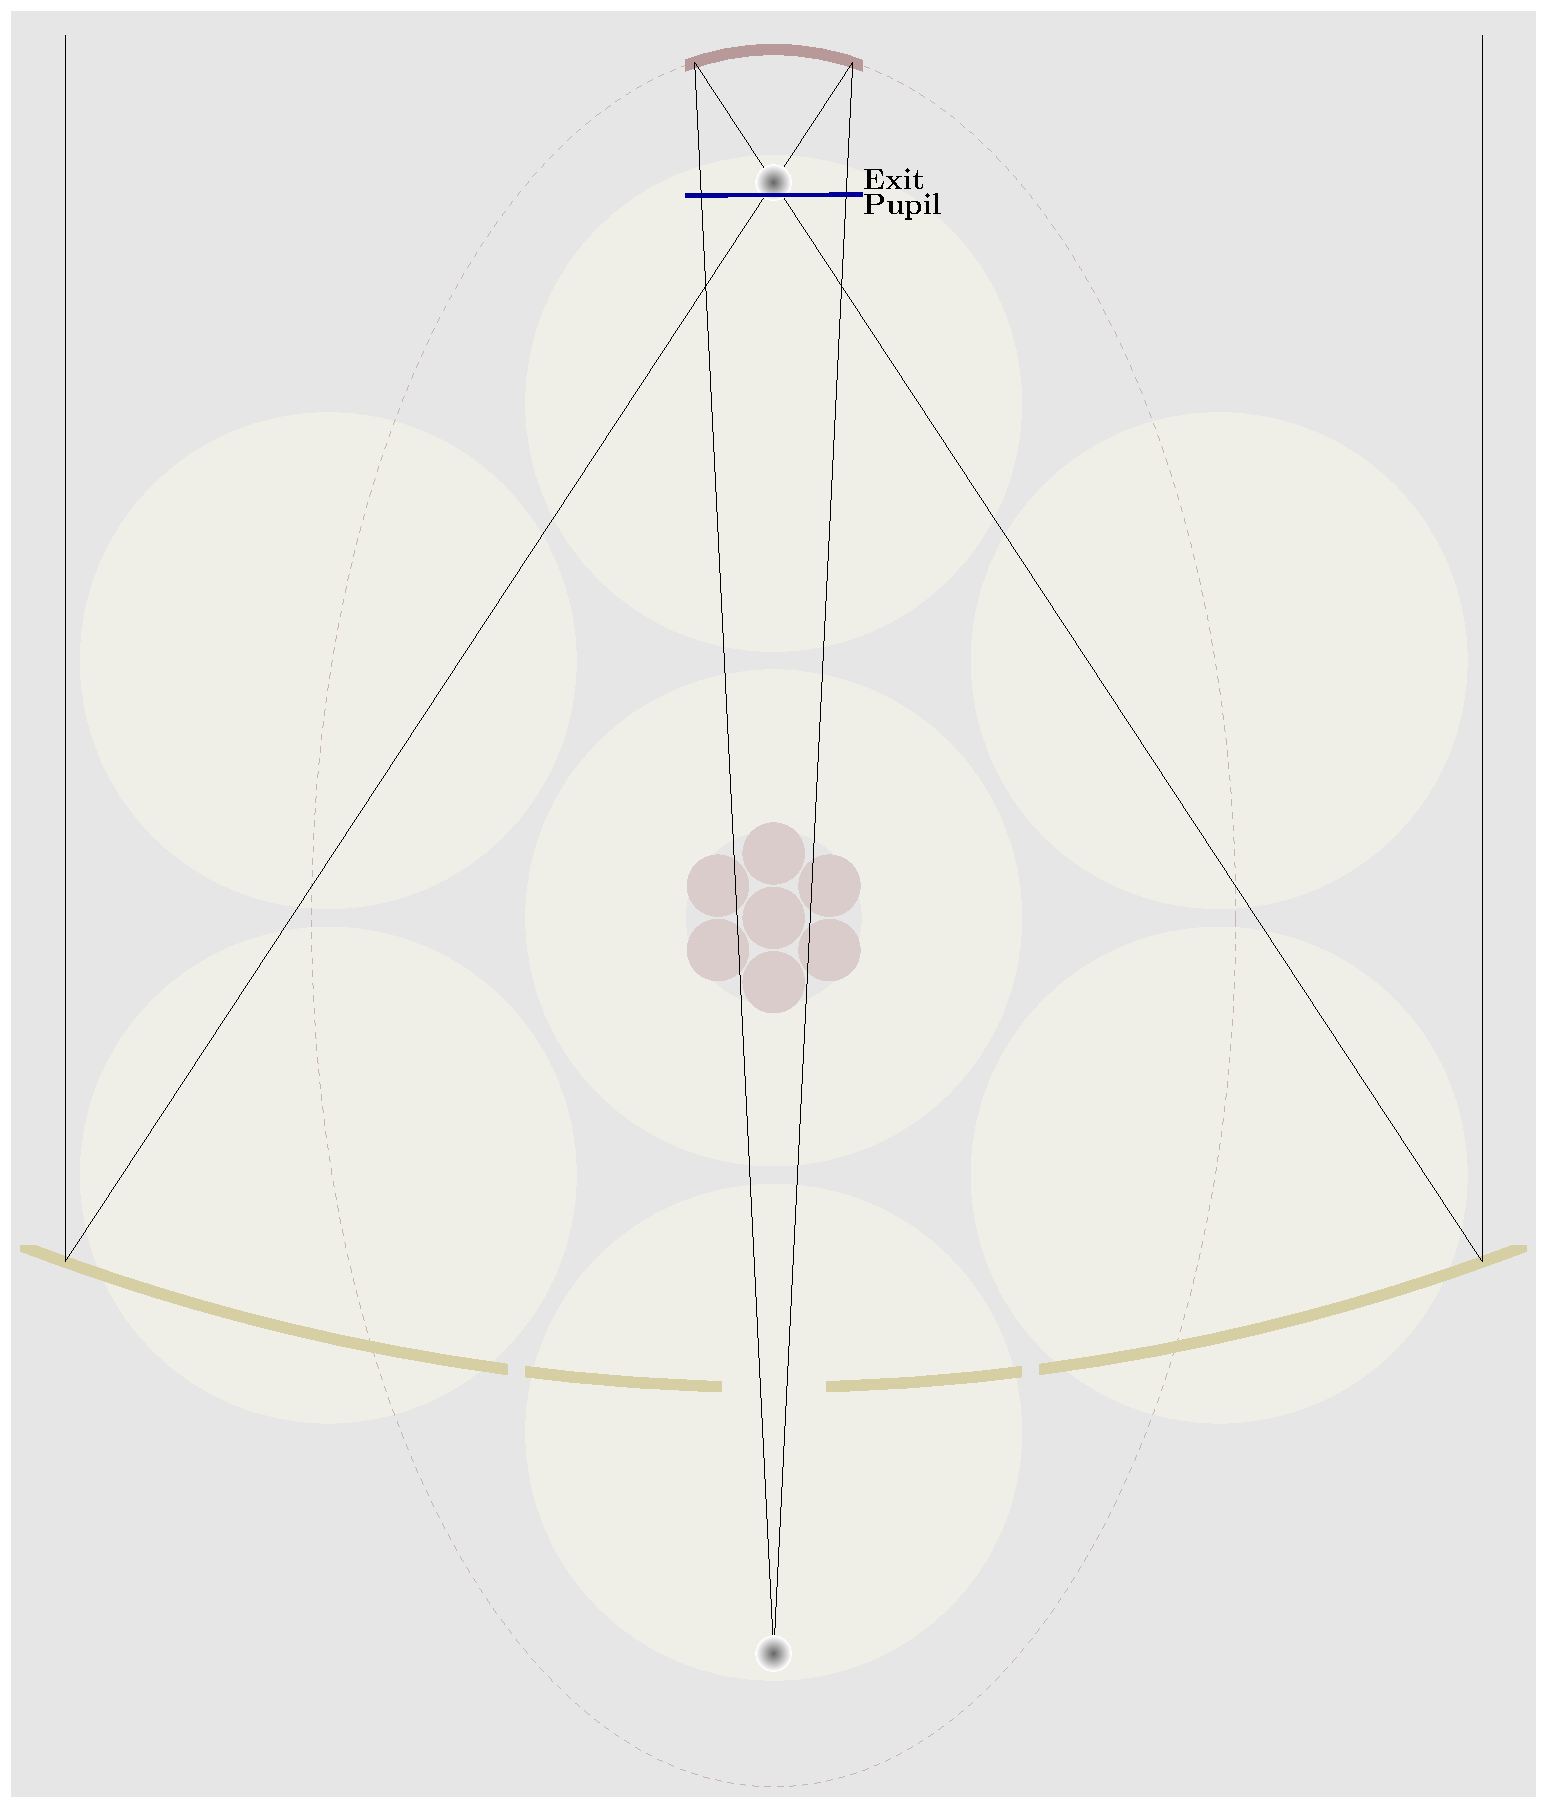
\includegraphics[width=0.6\linewidth]{./figures/ray_tracing.pdf}
   \caption{Ray tracing \& Fourier propagation.}
   \label{fig:12}
\end{figure}

\begin{figure}
   \centering
   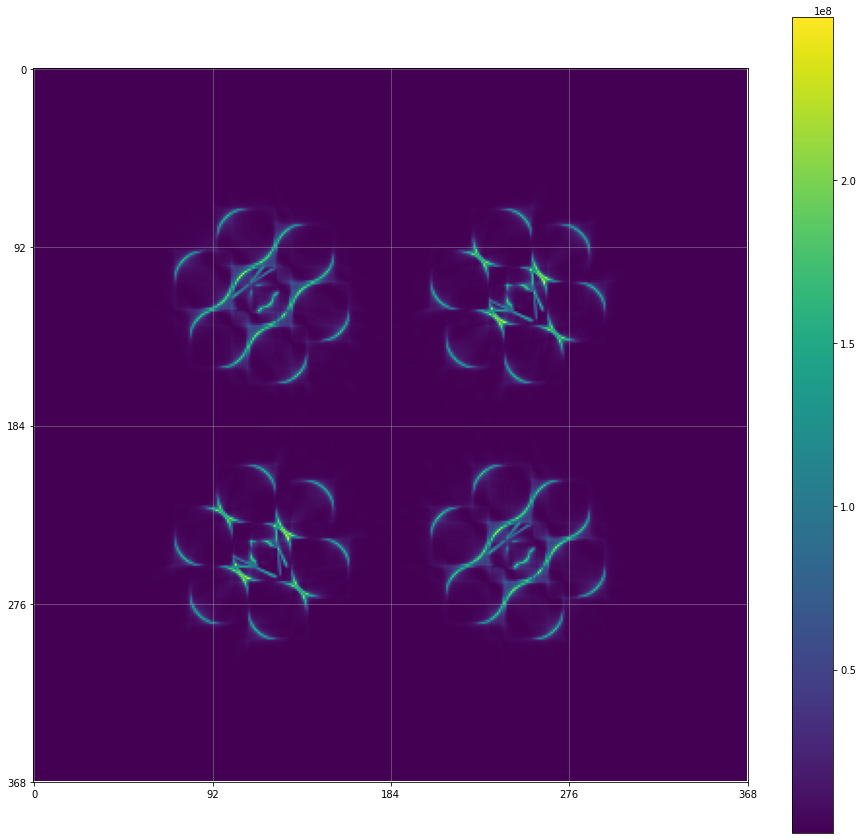
\includegraphics[trim=1cm 2cm 5cm 2cm,clip,width=0.6\linewidth]{./figures/pyramid.png}
   \caption{$96\times 96$ pyramid wavefront sensor.}
   \label{fig:13}
\end{figure}

\begin{figure}
   \centering
   \begin{tabular}{cc}
      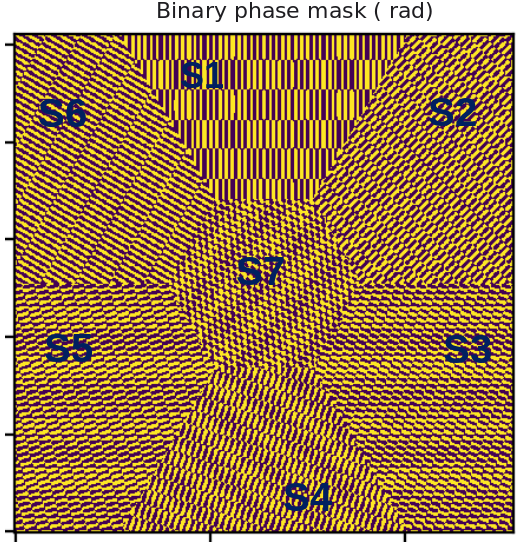
\includegraphics[width=0.4\linewidth]{./figures/hdfs_mask.png} &
      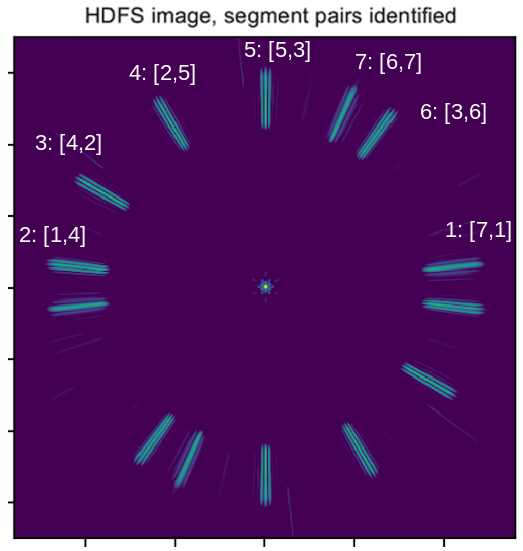
\includegraphics[width=0.4\linewidth]{./figures/hdfs_image.png}
   \end{tabular}
   \caption{Holographic dispersed fringe sensor (HDFS).}
   \label{fig:14}
\end{figure}

\clearpage

\subsection{Control Models}
\label{sec:control}

The complete control model of the NGAO Observing Mode of the GMT is given in Fig.~\ref{fig:15}.

\begin{figure}
   \centering
   \includegraphics[width=\linewidth]{./figures/{end2end_ngao-ngao-im-e2e.drawio}.pdf}
   \caption{Control Models.}
   \label{fig:15}
\end{figure}

\section{NGAO INTEGRATED MODEL COMPUTING FRAMEWORKS}
\label{sec:framework}

\subsection{Programming $\&$ Computing Challenges}
\label{sec:pc-challenge}

Building a NGAO integrated model for an extremely large telescope like the GMT presents unique software programming and computing challenges.

The dimensions of the model in terms of
\begin{itemize}
   \item degrees of freedom: $10^4$~modes, $10^4$~inputs \& $10^4$~outputs
   \item temporal sampling: $10^4$Hz
   \item science exposure: $10^3$s
\end{itemize}
leads to a dynamic model with millions of iterations where thousands of parameters are updated at each time step.
The model must also account for the multirate e.g.
\begin{itemize}
   \item 8kHz for structural model \& ASMS
   \item 100Hz for M1 control system
   \item 1kHz for Pyramid WFS
   \item 10Hz for Piston Sensor (HDFS)
\end{itemize}
and concurrent e.g.
\begin{itemize}
   \item segments (14) control system are independent
   \item actuators (M1 \& M2) run in parallel
\end{itemize}
nature of the telescope control system.

\subsection{Computing Framework Design}
\label{sec:framework-design}

From the considerations in the section above, the design of the integrated model
went through 4 stages:
\begin{itemize}
   \item Guiding Principle:
         \begin{itemize}
            \item low runtime, parallelizable
            \item scalable \& deployable at scale
         \end{itemize}
   \item Specifications:
         \begin{itemize}
            \item compiled language, async/thread API
            \item project tooling \& open source
         \end{itemize}
   \item Design:
         \begin{itemize}
            \item asynchronous, concurrent
                  \& distributed system
         \end{itemize}
   \item Solution \& Implementation:
         \begin{itemize}
            \item actors model
            \item Rust language
         \end{itemize}
\end{itemize}

\subsection{GMT NGAO Integrated Modeling}
\label{sec:gmt-ngao-im}

The final design of the integrated model computing framework implements the actors design pattern where
\begin{itemize}
   \item every block is an \emph{actor} interfacing with a \emph{client} i.e. a model (structural, optical, control, ...),
   \item actors run \emph{asynchronously} and communicate by \emph{exchanging} tagged \emph{data},
   \item actors \emph{synchronisation and sequencing} is the results of the actors \emph{network topology}.
\end{itemize}

Fig.~\ref{fig:16a} is an implementation of the Adaptive Optics block diagram of Fig.~\ref{fig:3} using the integrated model computing framework in the context of the GMT NGAO Observing mode.
Adding to the actors model of Fig.~\ref{fig:16a}, the structural dynamic model of the telescope and the control systems of the mount, M1 and M2 leads
to the new model depicted in Fig.~\ref{fig:16b}.


\begin{figure}
   \centering
   \includegraphics[width=0.8\linewidth]{./figures/{NGAO.dot}.png}
   \caption{NGAO Model with Atmospheric Turbulence.}
   \label{fig:16a}
\end{figure}

\begin{figure}
   \centering
   \includegraphics[width=\linewidth]{./figures/{ngao-opm.2pi}.png}
   \caption{Wind \& Turbulence (Atmosphere \& Dome Deeing) Loaded NGAO Integrated Model.}
   \label{fig:16b}
\end{figure}

\clearpage

\subsection{GMT Design Validation for NGAO Observations}
\label{sec:gmt-ngao-vv}

An application of the GMT NGAO Integrated Model is the compliance analysis of the NGAO optical performance with respect to the requirements under atmospheric turbulence, dome seeing and wind loads perturbations.
Using the CFD model described in Sec.~\ref{sec:cfd}, 60 CFD simulations were performed for
\begin{itemize}
   \item 4 wind speeds: 2m/s, 7m/s, 12m/s \& 17m/s
   \item 3 telescope elevations
         \begin{tabular}{ccc}
            90deg                                                             & 60deg & 30deg \\
            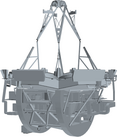
\includegraphics[width=0.2\linewidth]{./figures/zen00az000_OS7_tel_tr.png}  &
            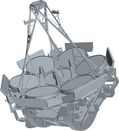
\includegraphics[width=0.2\linewidth]{./figures/zen30az000_CD12_tel_tr.png} &
            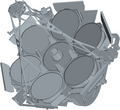
\includegraphics[width=0.2\linewidth]{./figures/zen60az000_CS17_tel_tr.png}
         \end{tabular}
   \item 3 enclosure settings
         \begin{tabular}{cccc}
            vents                                                         & open                                                         &
            closed                                                        &
            closed                                                                                                                         \\
            windscreen                                                    & stowed                                                       &
            deployed                                                      &
            stowed                                                                                                                         \\
                                                                          & 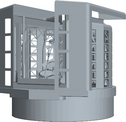
\includegraphics[width=0.2\linewidth]{./figures/zen30az000_OS7_tr.png} &
            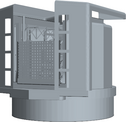
\includegraphics[width=0.2\linewidth]{./figures/zen30az000_CD12_tr.png} &
            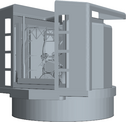
\includegraphics[width=0.2\linewidth]{./figures/zen60az000_CS17_tr.png}
         \end{tabular}.
\end{itemize}
Each simulation provides time series of dome seeing wavefront map in the telescope exit pupil and of forces and moments at various locations on the telescope structure.
For this compliance analysis, we are considering only the upwind cases reducing the set of CFD cases to 12 (Fig.~\ref{fig:17}).
\begin{figure}
   \centering
   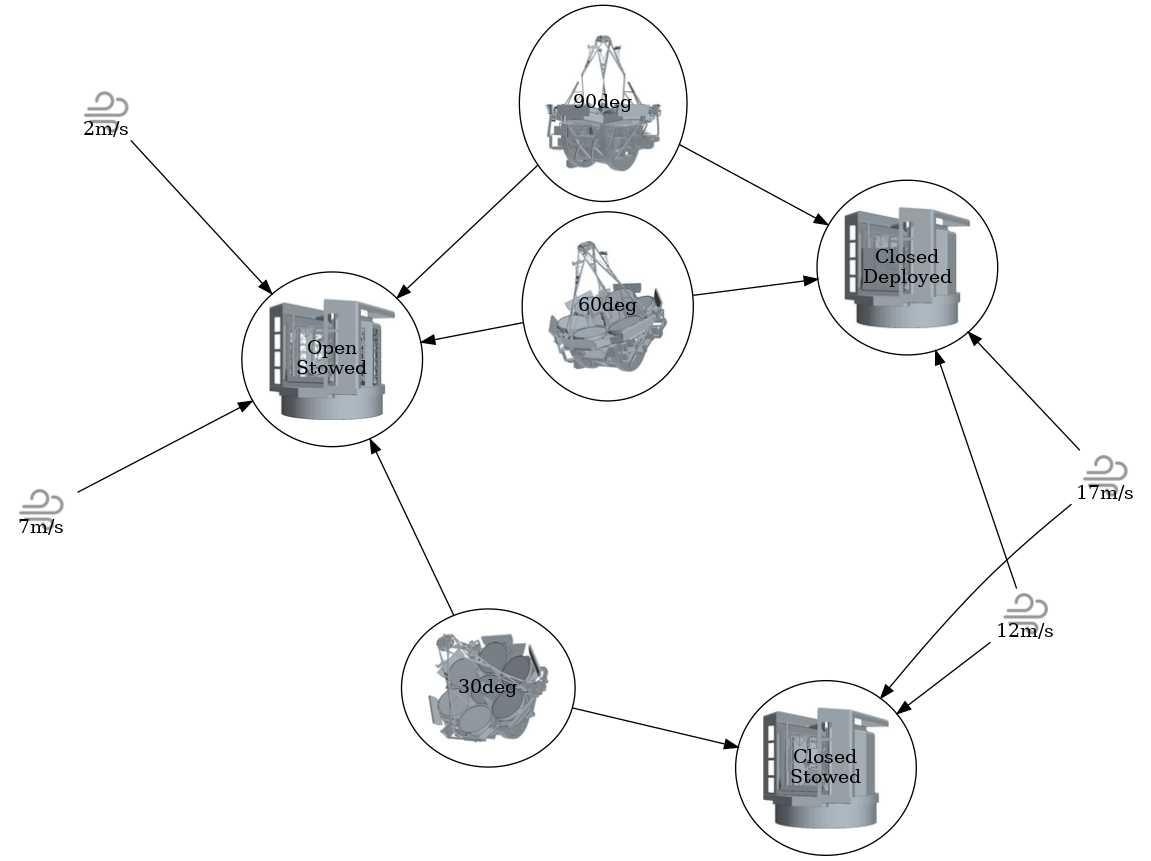
\includegraphics[width=\linewidth]{{./figures/cfd_cases_tr.dot}.png}
   \caption{12 possible CFD permutations.}
   \label{fig:17}
\end{figure}

The results of the 12 integrated modeling NGAO simulations are given in Figures~\ref{fig:18a}, \ref{fig:18b} and \ref{fig:18c}.
Each simulation is repeated 3 times, with the atmospheric turbulence only, with both atmospheric turbulence and dome seeing and with atmospheric turbulence, dome seeing and wind loads.
Each figure corresponds to a different telescope elevation and shows the WFE RMS as a function of wind speed.
The blue and orange areas highlights different enclosure configurations.
The lower bound of the areas marks the WFE RMS with atmospheric turbulence only and the upper bound marks the requirement value (only visible in Fig.~\ref{fig:18c}).
These simulations are re-done each time a design update (structural, control, ...) occurs.

\begin{figure}
   \centering
   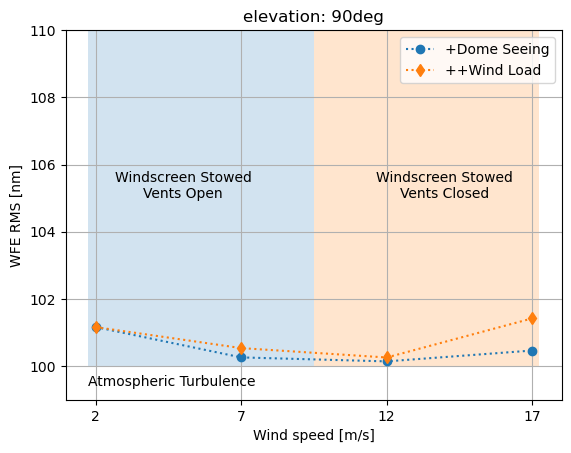
\includegraphics[width=0.5\linewidth]{./figures/wfe-rms_el90.png}
   \caption{Wavefront Error RMS as a function of wind speed and enclosure settings for 90deg GMT elevation.}
   \label{fig:18a}
\end{figure}

\begin{figure}
   \centering
   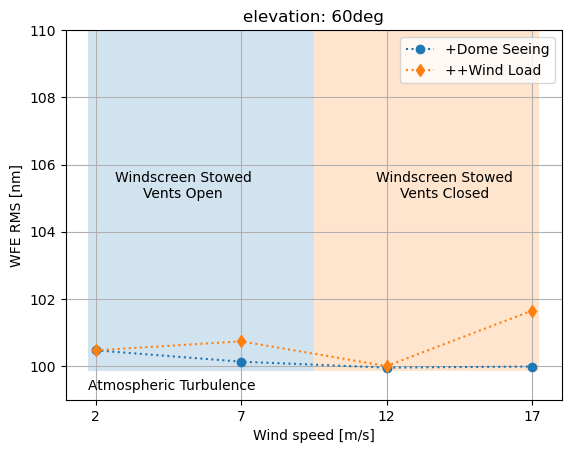
\includegraphics[width=0.5\linewidth]{./figures/wfe-rms_el60.png}
   \caption{Wavefront Error RMS as a function of wind speed and enclosure settings for 60deg GMT elevation.}
   \label{fig:18b}
\end{figure}

\begin{figure}
   \centering
   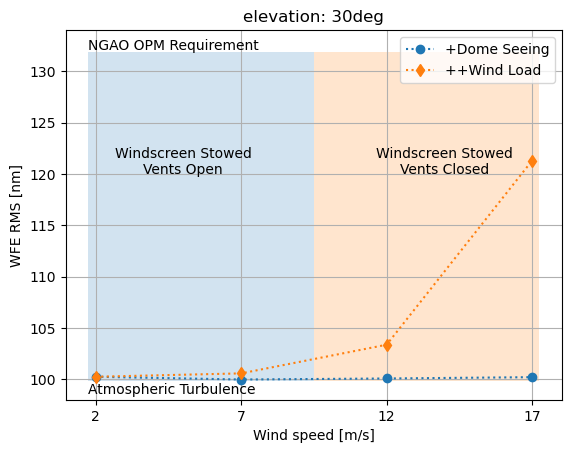
\includegraphics[width=0.5\linewidth]{./figures/wfe-rms_el30.png}
   \caption{Wavefront Error RMS as a function of wind speed and enclosure settings for 30deg GMT elevation.}
   \label{fig:18c}
\end{figure}

\clearpage

\section{CONCLUSION}
\label{sec:conclusion}

\begin{itemize}
   \item ELT end-to-end modeling, with Adaptive Optics, is now feasible
   \item ELT structural dynamic properties are very relevant to the performance of all the Adaptive Optics mode of operations
         \begin{itemize}
            \item that includes modeling the effects of wind buffeting
         \end{itemize}
   \item the GMT Integrated Modeling Framework is a very potent tool to perform systemic trade study \& design validation
   \item the next challenge is the Integrated Model of the GMT Laser Tomography Adaptive Optics System
\end{itemize}

%\printbibliography %Prints bibliography
\end{document}
